\section{实验要求与实验目的}

\subsection{实验要求}
本实验要求在 Proteus 中搭建以 AT89C51 和 DAC0832 为核心的波形发生器。单片机通过并行口向 DAC0832 输出 8 位数字量，经运算放大器转换为模拟电压，并在示波器上观察输出波形。基本要求如下：
\begin{enumerate}
  \item 使用 AT89C51 的 P0 口连接 DAC0832 的 DI0--DI7，完成 8 位数字量到模拟量的转换。
  \item 使用 P1.0--P1.3 的拨码开关选择方波、锯齿波、三角波和正弦波四种输出波形。
  \item 使用 P1.4--P1.7 的 LED 指示当前选中的波形，LED 采用低电平有效方式驱动。
  \item 使用 P2 口作为频率选择输入，通过改变 P2 口拨码值调节软件延时，从而改变输出波形频率。
\end{enumerate}

在完成基本功能的基础上，实验还包含以下拓展要求：
\begin{enumerate}
  \item 在 Proteus 中完整呈现单片机最小系统、DAC0832 接口、运放输出、波形选择和频率选择电路。
  \item 对四种波形分别进行仿真截图，证明输出波形形状与程序设计相符。
  \item 对不同 P2 输入下的波形频率进行对比，说明频率控制功能有效。
\end{enumerate}

\subsection{实验目的}
\begin{enumerate}
  \item 掌握 AT89C51 并行 I/O 口输出数字量、读取拨码输入以及驱动 LED 指示电路的方法。
  \item 理解 DAC0832 的数字量输入、参考电压和运算放大器电流-电压转换输出原理。
  \item 掌握用软件查表和循环计数生成周期波形的方法，并分析软件延时对频率的影响。
  \item 提高 Proteus 环境下单片机、D/A 转换器和虚拟示波器联合调试的能力。
\end{enumerate}

\subsection{总体设计思路}
系统以 AT89C51 为控制核心，P0 口作为波形数据总线，直接把 8 位采样值送入 DAC0832。DAC0832 工作在直通转换方式，片选和写控制信号固定为有效状态，P0 口数据变化后即可在模拟输出端体现为对应电压。P1 口低四位连接波形选择拨码开关，程序每输出一个周期后重新扫描按键；P1 口高四位连接 LED，用于指示当前波形。P2 口连接 8 位拨码开关作为频率控制量，程序将其取反后作为延时循环次数，因此 P2 值越大，延时越短，输出频率越高。

\section{Proteus 原理图与硬件电路说明}

\subsection{完整原理图}
\begin{figure}[H]
  \centering
  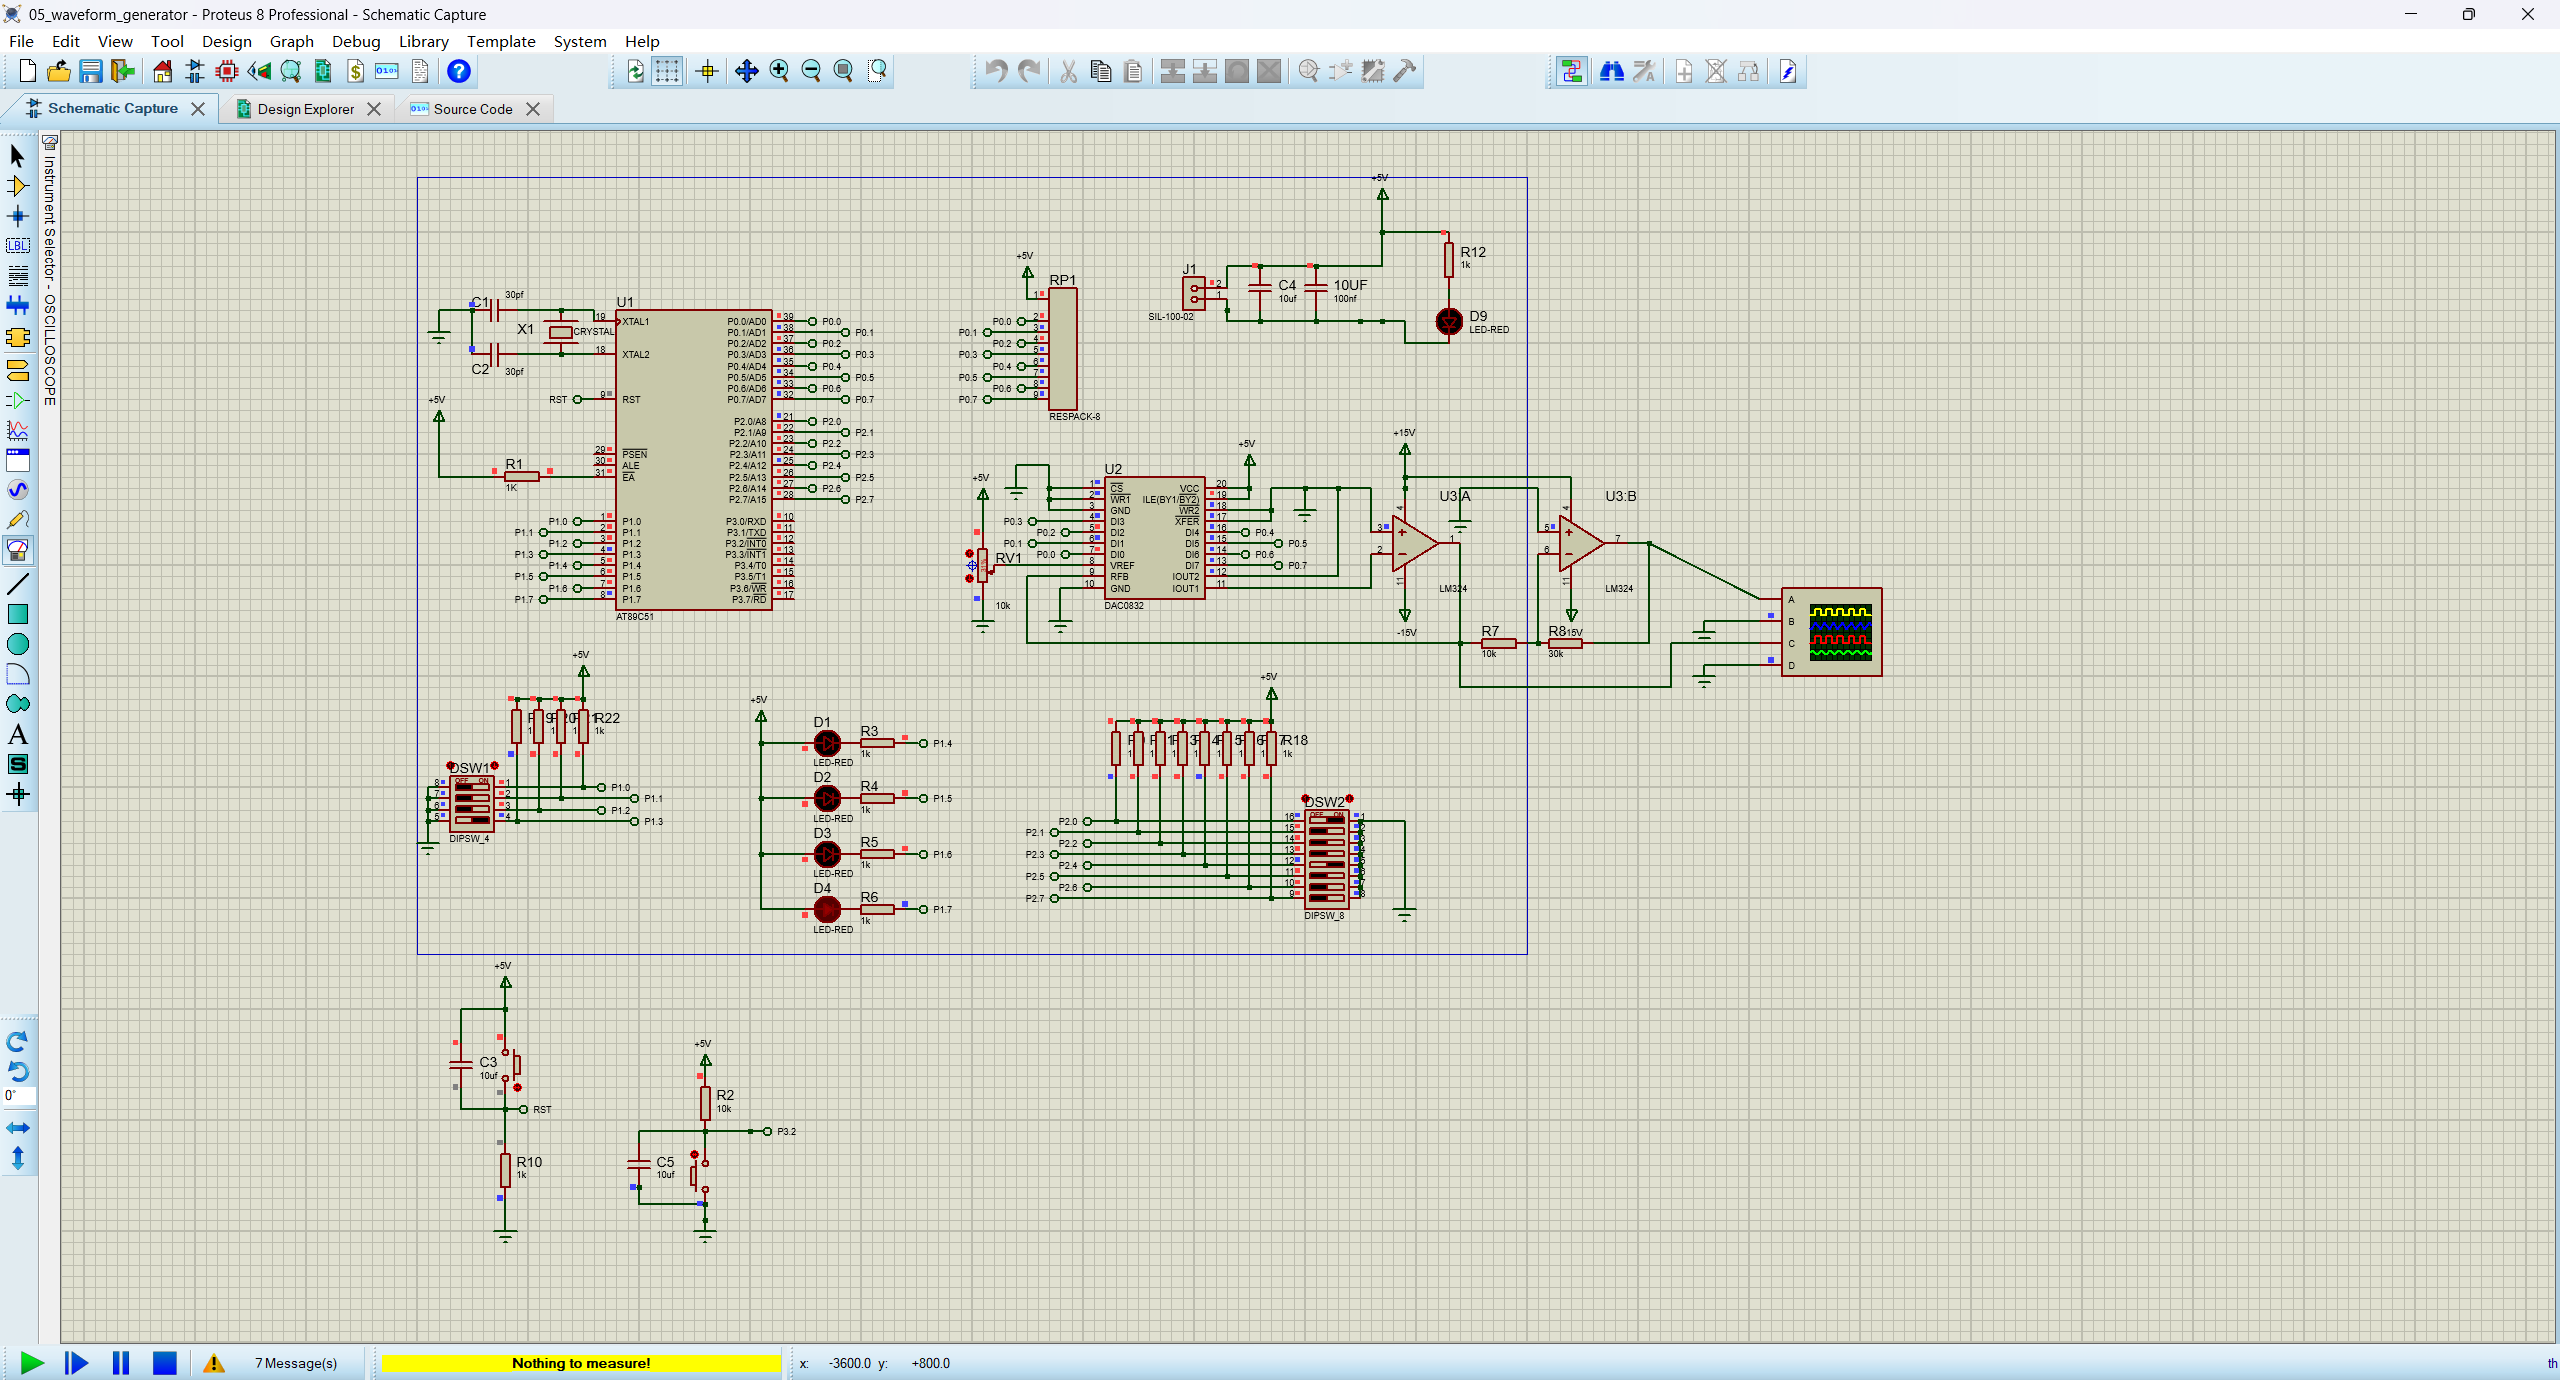
\includegraphics[width=0.95\textwidth]{images/ProteusSchematic.png}
  \caption{实验六波形发生器 Proteus 完整原理图}
\end{figure}

完整电路由 AT89C51 最小系统、DAC0832 数模转换模块、LM324 运算放大器输出模块、P1 口波形选择与 LED 指示模块、P2 口频率选择模块组成。数字部分使用 +5V 供电，运放部分采用正负电源供电，以便输出端能够获得较好的模拟波形摆幅。

\subsection{单片机最小系统}
\begin{figure}[H]
  \centering
  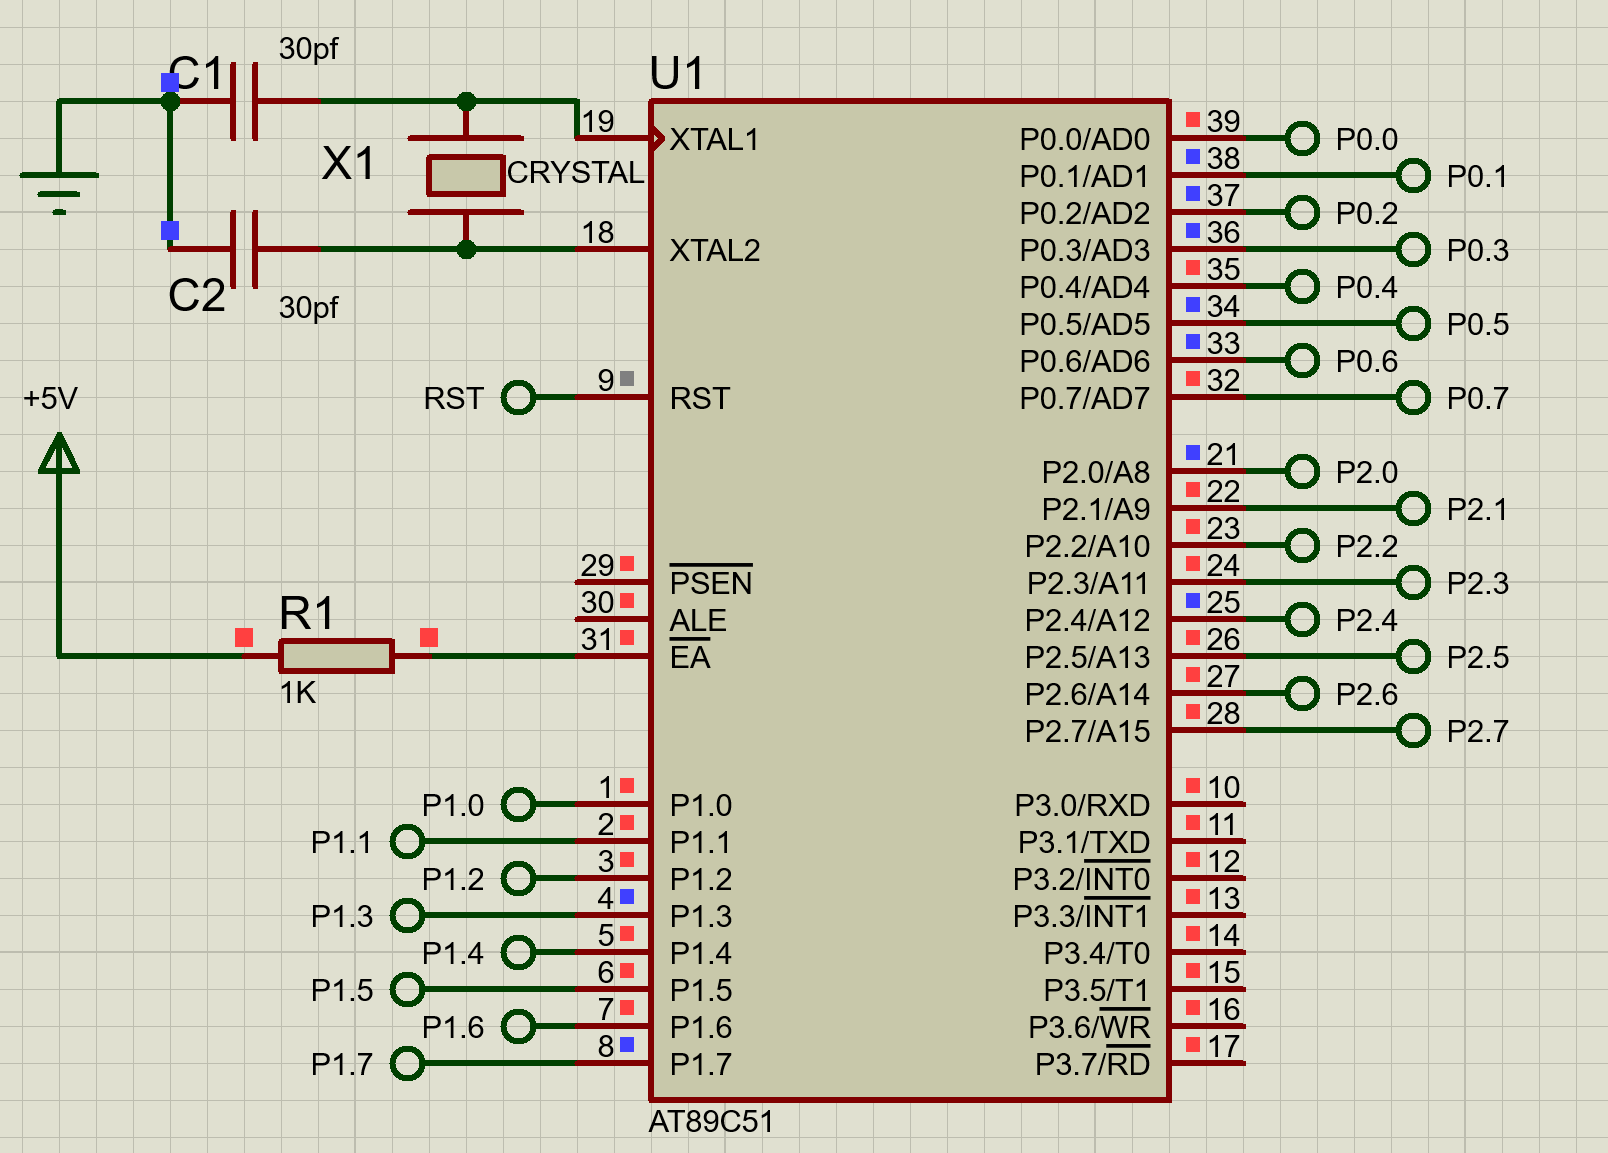
\includegraphics[width=0.70\textwidth]{images/power.png}
  \caption{AT89C51 供电与 12MHz 晶振电路}
\end{figure}

AT89C51 的 VCC 与 GND 接入 +5V 电源和公共地，XTAL1、XTAL2 外接 12MHz 晶振，并配合两个 30pF 电容构成时钟振荡电路。12MHz 晶振下，8051 一个机器周期约为 1us，便于通过软件循环估算延时时间。

\begin{figure}[H]
  \centering
  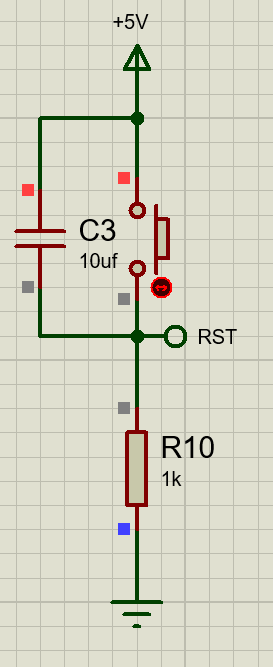
\includegraphics[width=0.55\textwidth]{images/rst.png}
  \caption{单片机复位电路}
\end{figure}

复位电路由按键、电阻和电容构成。上电时电容充电产生短暂高电平，按下复位键时 RST 引脚被拉到有效电平，使程序从 0000H 复位向量重新开始执行。

\subsection{DAC0832 与模拟输出电路}
\begin{figure}[H]
  \centering
  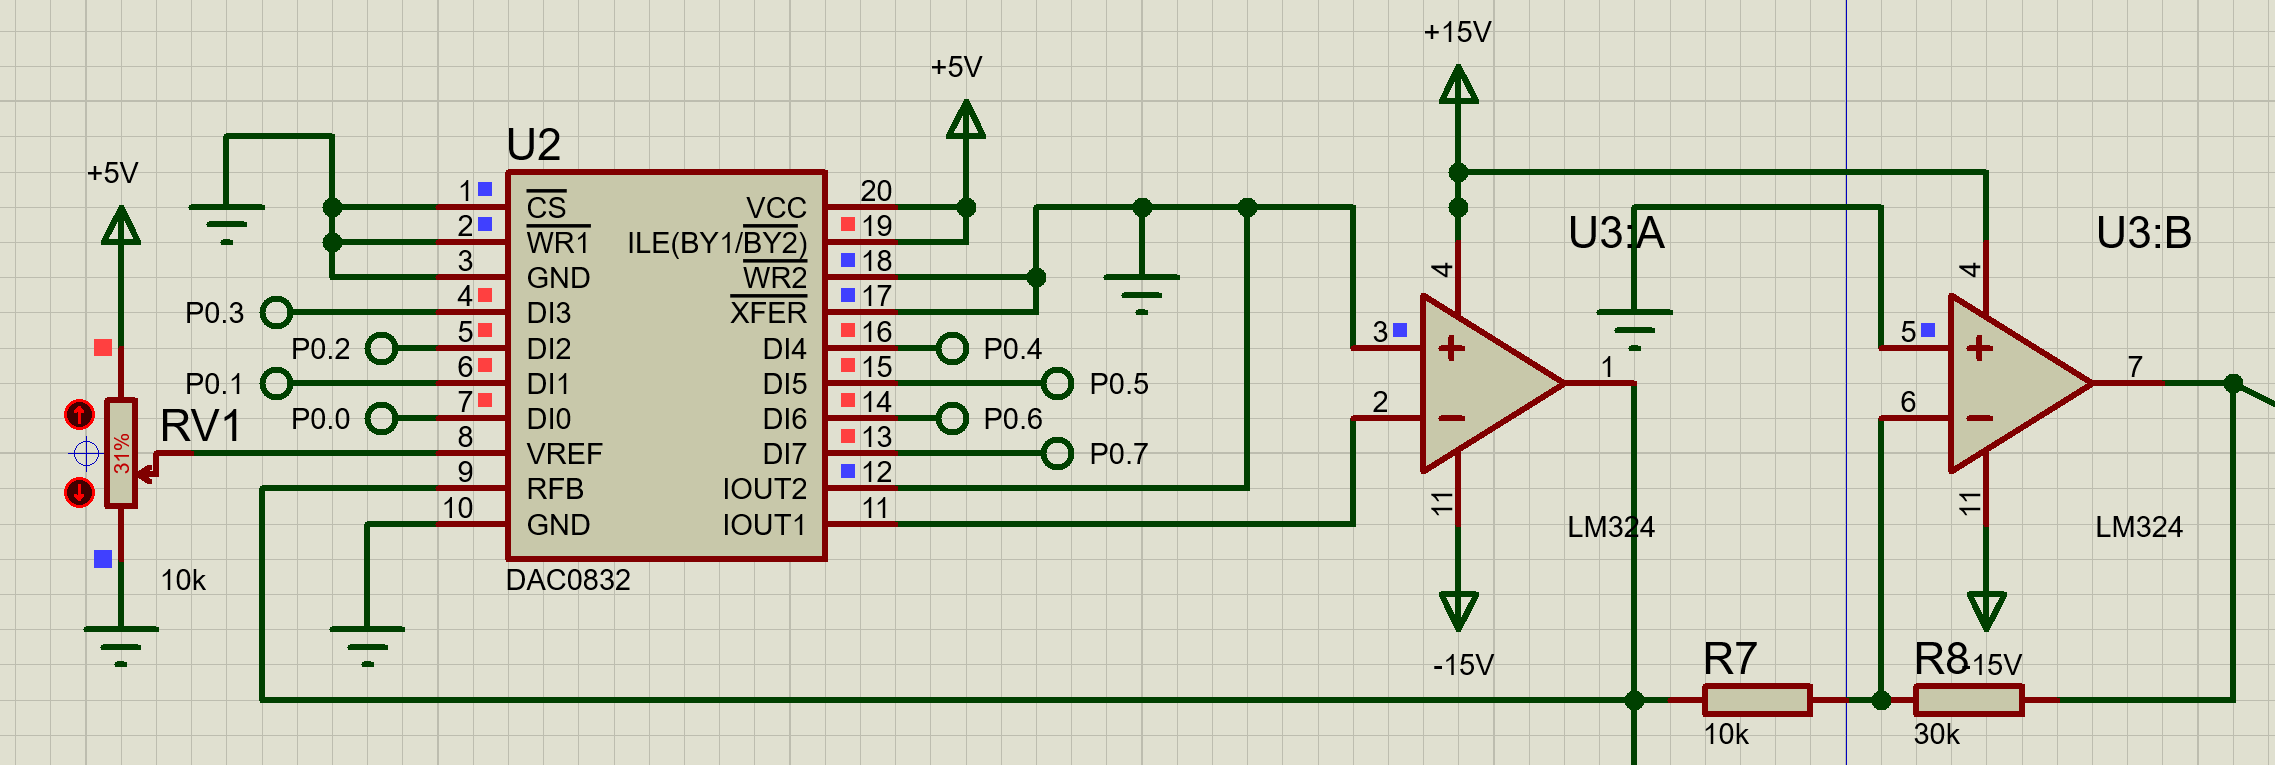
\includegraphics[width=0.86\textwidth]{images/dac_circuit.png}
  \caption{DAC0832 与 LM324 运放输出电路}
\end{figure}

DAC0832 的 DI0--DI7 与 AT89C51 的 P0.0--P0.7 相连，作为 8 位并行输入数据总线。电路中 CS、WR1、WR2、XFER 等控制端固定为有效状态，使 DAC0832 处于直通工作方式。单片机写入 P0 的数据不需要额外片选脉冲，即可进入 D/A 转换链路。参考电压由电位器调节，输出电流经 LM324 运算放大器转换为电压信号，最终送到示波器或模拟波形图进行观察。

\subsection{波形选择与 LED 指示电路}
\begin{figure}[H]
  \centering
  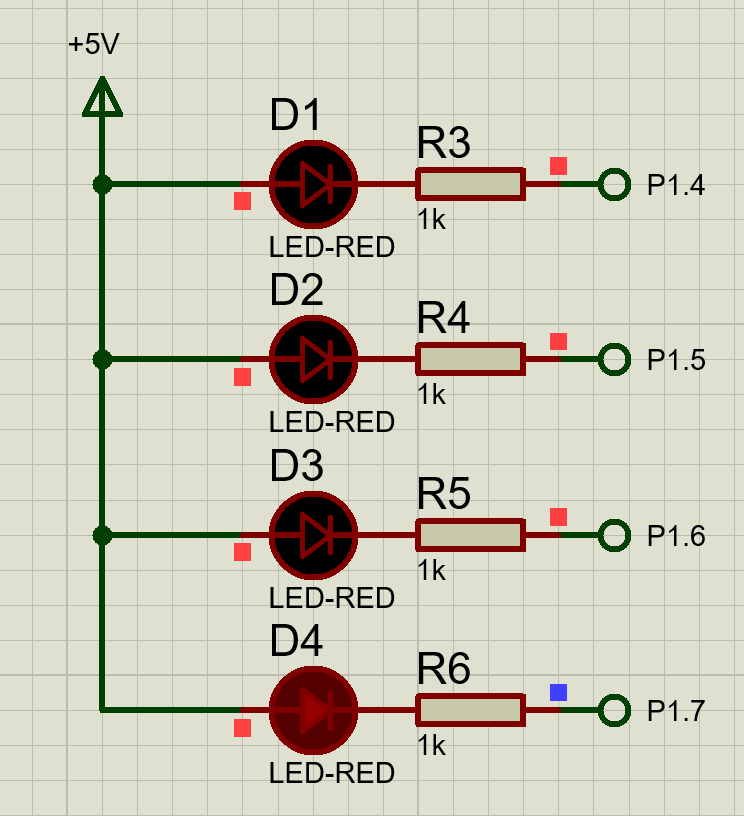
\includegraphics[width=0.74\textwidth]{images/led_key.png}
  \caption{P1 口波形选择拨码开关与 LED 指示电路}
\end{figure}

P1.0--P1.3 分别对应方波、锯齿波、三角波和正弦波选择输入，拨码开关闭合时相应引脚为低电平。P1.4--P1.7 分别连接四个 LED，程序输出低电平点亮相应指示灯。由于 P1 口同一端口同时承担输入和输出功能，程序在点亮 LED 时保持低四位为高电平，避免影响下一次按键扫描。

\begin{figure}[H]
  \centering
  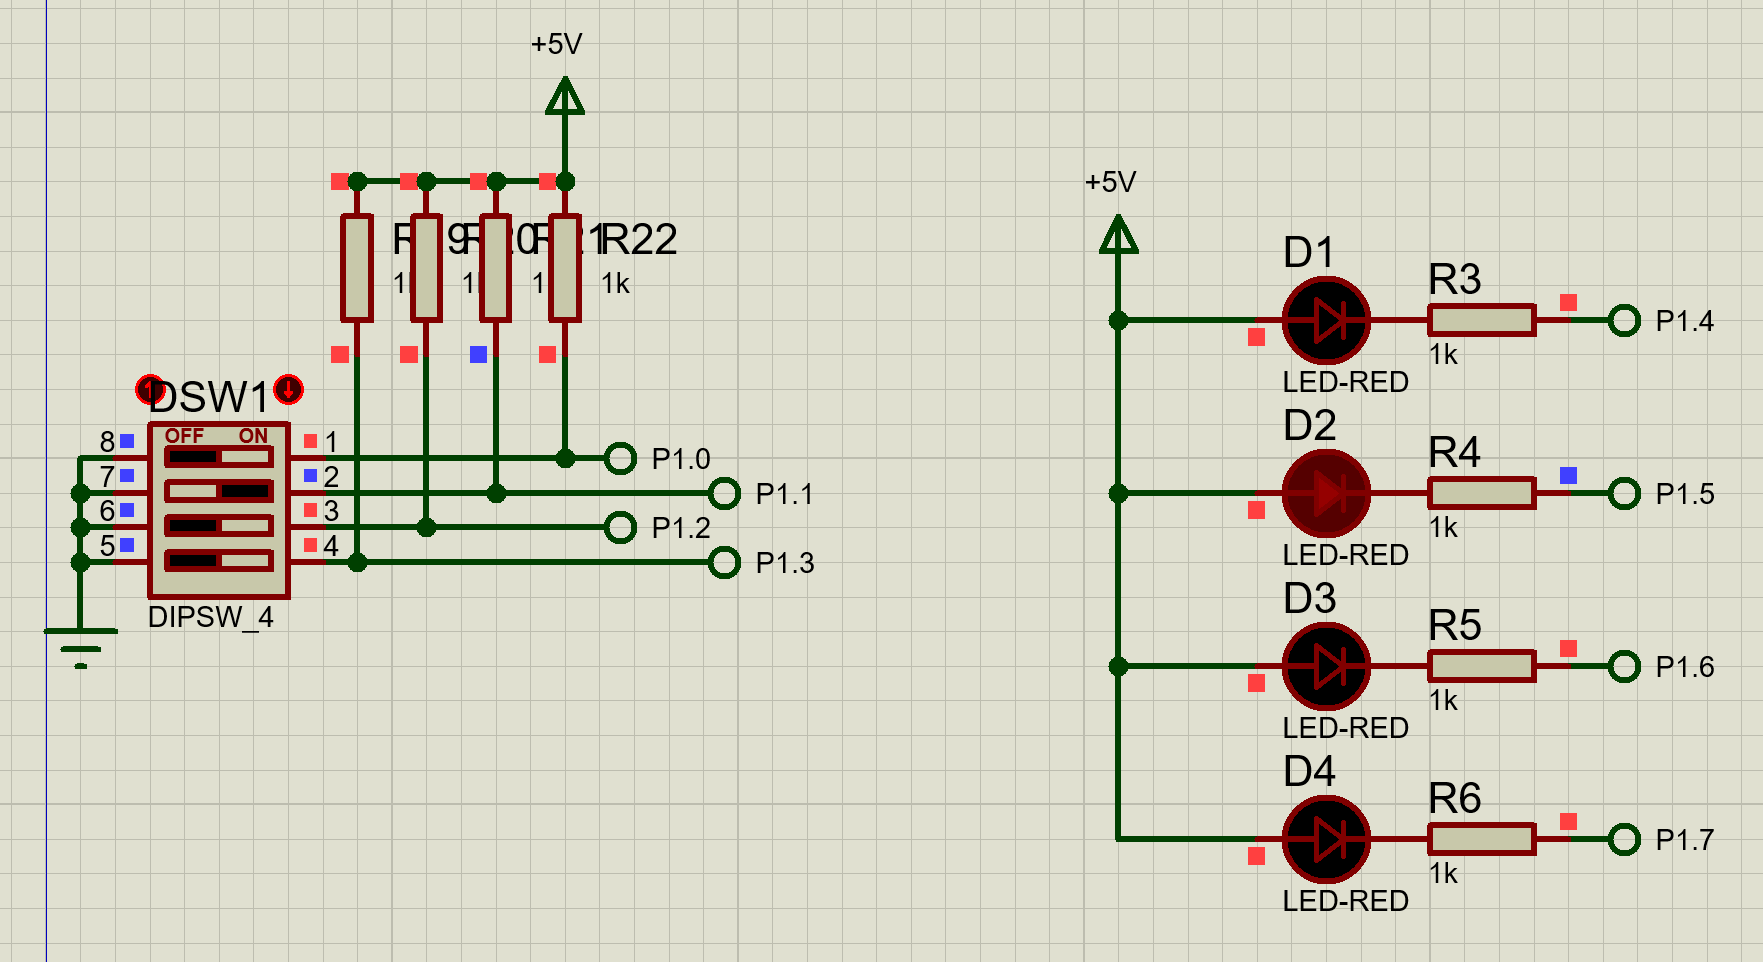
\includegraphics[width=0.58\textwidth]{images/led.png}
  \caption{波形指示 LED 点亮状态}
\end{figure}

\subsection{频率选择电路}
\begin{figure}[H]
  \centering
  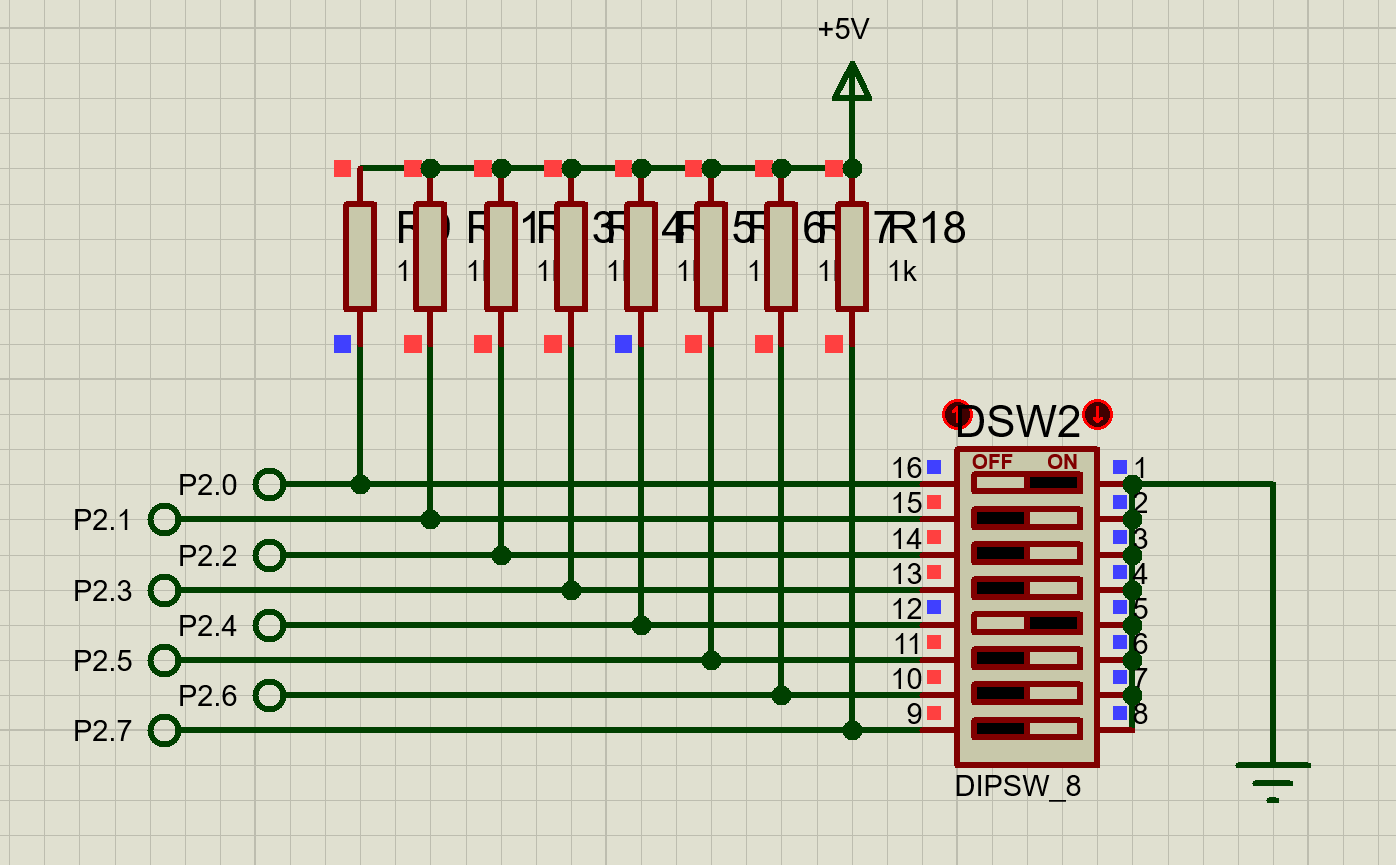
\includegraphics[width=0.72\textwidth]{images/freq_switch.png}
  \caption{P2 口 8 位频率选择拨码开关}
\end{figure}

P2.0--P2.7 连接 DIPSW\_8 作为频率输入。程序在延时函数中读取 P2，然后执行取反操作，得到软件延时循环次数。当 P2 值较小时，取反后的延时值较大，波形周期较长；当 P2 值较大时，延时值较小，波形周期缩短。

\subsection{主要元件清单}
\begin{table}[H]
  \centering
  \caption{实验六主要元件与功能}
  \small
  \renewcommand{\arraystretch}{1.3}
  \begin{tabular}{cp{0.18\textwidth}p{0.20\textwidth}p{0.42\textwidth}}
    \toprule
    序号 & 元件名称 & 型号或规格 & 功能说明 \\
    \midrule
    1 & 单片机 & AT89C51 & 读取拨码开关，输出波形采样值，控制 LED 指示 \\
    2 & 数模转换器 & DAC0832 & 将 P0 口 8 位数字量转换为模拟电流输出 \\
    3 & 运算放大器 & LM324 & 完成电流-电压转换及模拟电压输出 \\
    4 & 晶振 & 12MHz & 提供单片机运行时钟 \\
    5 & 电位器 & POT-HG & 调节 DAC0832 参考电压，影响输出幅度 \\
    6 & 拨码开关 & DIPSW & P1 选择波形，P2 调节频率 \\
    7 & LED 与电阻 & LED / RES & 指示当前输出波形并限制 LED 电流 \\
    8 & 示波器或波形图 & OSCILLOSCOPE / GRAPH & 观察运放输出端模拟波形 \\
    \bottomrule
  \end{tabular}
\end{table}

\section{软件设计与程序流程}

\subsection{端口分配}
\begin{table}[H]
  \centering
  \caption{AT89C51 端口分配表}
  \renewcommand{\arraystretch}{1.35}
  \begin{tabular}{p{0.22\textwidth}p{0.30\textwidth}p{0.38\textwidth}}
    \toprule
    端口 & 连接对象 & 软件作用 \\
    \midrule
    P0.0--P0.7 & DAC0832 DI0--DI7 & 输出 8 位波形采样值 \\
    P1.0 & 方波选择开关 & 低电平有效，返回波形编号 00H \\
    P1.1 & 锯齿波选择开关 & 低电平有效，返回波形编号 01H \\
    P1.2 & 三角波选择开关 & 低电平有效，返回波形编号 02H \\
    P1.3 & 正弦波选择开关 & 低电平有效，返回波形编号 03H \\
    P1.4--P1.7 & 四个 LED 指示灯 & 低电平点亮，显示当前波形 \\
    P2.0--P2.7 & 频率选择拨码开关 & 输入延时调节量，P2 越大频率越高 \\
    \bottomrule
  \end{tabular}
\end{table}

\subsection{主程序流程}
\begin{figure}[H]
\centering
\resizebox{\textwidth}{!}{%
\begin{tikzpicture}[
  node distance=8mm and 13mm,
  proc/.style={rectangle,rounded corners,draw=themecolor,fill=blue!3,minimum width=5.9cm,minimum height=8mm,align=center},
  io/.style={trapezium,trapezium left angle=75,trapezium right angle=105,draw=themecolor,fill=cyan!6,minimum width=5.9cm,minimum height=8mm,align=center},
  decision/.style={diamond,aspect=2.2,draw=accentyellow,fill=yellow!9,minimum width=4.6cm,minimum height=10mm,align=center},
  line/.style={-Latex,thick,draw=themecolor}
]
  \node[proc] (start) {程序复位，设置堆栈指针};
  \node[proc,below=of start] (init) {P0 清零，P1/P2 写 0FFH 释放输入锁存};
  \node[io,below=of init] (scan) {扫描 P1.0--P1.3，获得波形编号};
  \node[decision,below=of scan] (choose) {判断波形编号};
  \node[proc,below left=11mm and 25mm of choose] (square) {输出一个周期方波};
  \node[proc,below=11mm of choose] (saw) {输出一个周期锯齿波};
  \node[proc,below right=11mm and 25mm of choose] (tri) {输出一个周期三角波};
  \node[proc,below=16mm of saw] (sine) {输出一个周期正弦波};

  \draw[line] (start) -- (init);
  \draw[line] (init) -- (scan);
  \draw[line] (scan) -- (choose);
  \draw[line] (choose) -- node[left,font=\small] {00H} (square);
  \draw[line] (choose) -- node[right,font=\small] {01H} (saw);
  \draw[line] (choose) -- node[right,font=\small] {02H} (tri);
  \draw[line] (choose) |- node[right,font=\small,pos=0.25] {03H} (sine);
  \draw[line] (square.west) -- ++(-0.9,0) |- (scan.west);
  \draw[line] (saw.east) -- ++(1.0,0) |- (scan.east);
  \draw[line] (tri.east) -- ++(1.0,0) |- (scan.east);
  \draw[line] (sine.west) -- ++(-1.2,0) |- (scan.west);
\end{tikzpicture}
}
\caption{波形发生器主程序流程图}
\end{figure}

主程序采用循环扫描方式。每次调用对应波形子程序时只输出一个完整周期，周期结束后返回主循环重新读取 P1 低四位。这样设计的好处是按键切换不需要中断支持，程序结构清晰，且能够在一个周期结束后稳定切换到新的波形。

\subsection{四种波形生成方法}
\begin{table}[H]
  \centering
  \caption{四种波形的软件生成方法}
  \renewcommand{\arraystretch}{1.35}
  \begin{tabular}{p{0.16\textwidth}p{0.28\textwidth}p{0.46\textwidth}}
    \toprule
    波形 & 输出规律 & 程序实现 \\
    \midrule
    方波 & 00H 与 FFH 交替输出 & 低电平保持半周期，高电平保持半周期，形成高低电平交替 \\
    锯齿波 & 00H 到 FFH 单调递增 & 累加器从 00H 自增到溢出，每步输出一次并延时 \\
    三角波 & 00H 到 FFH 再回到 00H & 先执行递增输出，再执行递减输出，形成线性上升和下降 \\
    正弦波 & 以 80H 为中心上下变化 & 读取四分之一正弦表，通过对称和取反生成完整周期 \\
    \bottomrule
  \end{tabular}
\end{table}

\subsection{正弦波查表流程}
\begin{figure}[H]
\centering
\begin{tikzpicture}[
  node distance=8mm,
  proc/.style={rectangle,rounded corners,draw=themecolor,fill=blue!3,minimum width=7.2cm,minimum height=8mm,align=center},
  calcnode/.style={rectangle,rounded corners,draw=accentgreen,fill=green!8,minimum width=7.2cm,minimum height=8mm,align=center},
  line/.style={-Latex,thick,draw=themecolor}
]
  \node[proc] (dptr) {DPTR 指向 92 点四分之一正弦表};
  \node[calcnode,below=of dptr] (q1) {第一象限：表值 + 80H，输出中点以上曲线};
  \node[calcnode,below=of q1] (q2) {第二象限：反向读取表值 + 80H，输出对称曲线};
  \node[calcnode,below=of q2] (q3) {第三象限：80H - 表值，输出中点以下曲线};
  \node[calcnode,below=of q3] (q4) {第四象限：反向读取并执行 80H - 表值};
  \node[proc,below=of q4] (ret) {完整周期结束，返回主循环重新扫描波形选择};

  \draw[line] (dptr) -- (q1);
  \draw[line] (q1) -- (q2);
  \draw[line] (q2) -- (q3);
  \draw[line] (q3) -- (q4);
  \draw[line] (q4) -- (ret);
\end{tikzpicture}
\caption{正弦波查表与对称生成流程图}
\end{figure}

正弦表中仅保存从 0 到峰值的四分之一周期幅值，范围为 00H--7FH。程序输出时以 80H 作为中心值，前两个象限采用加法生成上半周，后两个象限采用减法生成下半周。与直接存储完整周期相比，这种方法节省了代码空间，同时保证输出曲线平滑。

\subsection{延时与频率控制}
延时函数 \texttt{STEP\_DELAY} 是频率控制的核心。程序读取 P2 后先取反，得到 \texttt{255 - P2}，再作为 R6 的循环次数。若 P2 为 FFH，取反结果为 00H，程序通过 \texttt{INC A} 保证仍有最小延时。其关系可概括为：
\[
  T_{\text{step}} \propto 255 - P2
\]
因此 P2 值越大，每个采样点之间的间隔越短；波形每周期采样点数不变时，周期缩短，频率升高。方波使用 \texttt{HALF\_DELAY} 形成半周期延时，锯齿波、三角波和正弦波则在每个采样点后调用 \texttt{STEP\_DELAY}。

\subsection{完整实验代码}
\lstset{style=a51style}
\lstinputlisting[caption={06\_waveform\_generator.A51 完整源代码}]{code/06_waveform_generator.A51}

\subsection{关键代码说明}
\begin{table}[H]
  \centering
  \caption{关键程序段与功能说明}
  \renewcommand{\arraystretch}{1.35}
  \begin{tabular}{p{0.34\textwidth}p{0.58\textwidth}}
    \toprule
    指令或程序段 & 功能说明 \\
    \midrule
    \texttt{MOV P0,\#00H} & 初始化 DAC 输入数据，使模拟输出从低电平开始。 \\
    \texttt{MOV P2,\#0FFH} & 向 P2 写 1，释放准双向口输入锁存，便于读取拨码开关。 \\
    \texttt{MOV P1,\#0FFH} & 释放 P1 低四位输入，同时关闭高四位 LED。 \\
    \texttt{ANL A,\#0FH} & 只保留 P1.0--P1.3 的波形选择输入。 \\
    \texttt{JNB ACC.0,KEY\_SQUARE} & 检测低电平有效的方波选择开关。 \\
    \texttt{MOV P1,\#0EFH} & P1.4 输出低电平，点亮方波指示 LED。 \\
    \texttt{INC A / JNZ SAW\_LOOP} & 锯齿波从 00H 递增到 FFH，溢出后结束一个周期。 \\
    \texttt{MOVC A,@A+DPTR} & 按偏移量读取程序存储器中的正弦表数据。 \\
    \texttt{CPL A} & 将 P2 输入取反，把较大的 P2 值转换为较短的软件延时。 \\
    \bottomrule
  \end{tabular}
\end{table}

\section{调试过程与实验结果}

\subsection{调试步骤}
\begin{enumerate}
  \item 检查 AT89C51 的 VCC、GND、晶振和复位连接，确认单片机能够正常启动。
  \item 检查 P0 到 DAC0832 DI0--DI7 的连接顺序，避免位序接反导致波形幅值异常。
  \item 确认 DAC0832 控制端处于直通有效状态，LM324 供电和反馈连接正确。
  \item 将汇编程序加载到 AT89C51，运行仿真后先观察默认方波输出。
  \item 依次切换 P1.0--P1.3 拨码开关，观察四个 LED 指示状态和示波器波形。
  \item 保持同一种波形，改变 P2 口拨码值，比较低频、中频和高频时波形周期变化。
\end{enumerate}

\subsection{四种输出波形}
\begin{figure}[H]
  \centering
  \begin{subfigure}{0.48\textwidth}
    \centering
    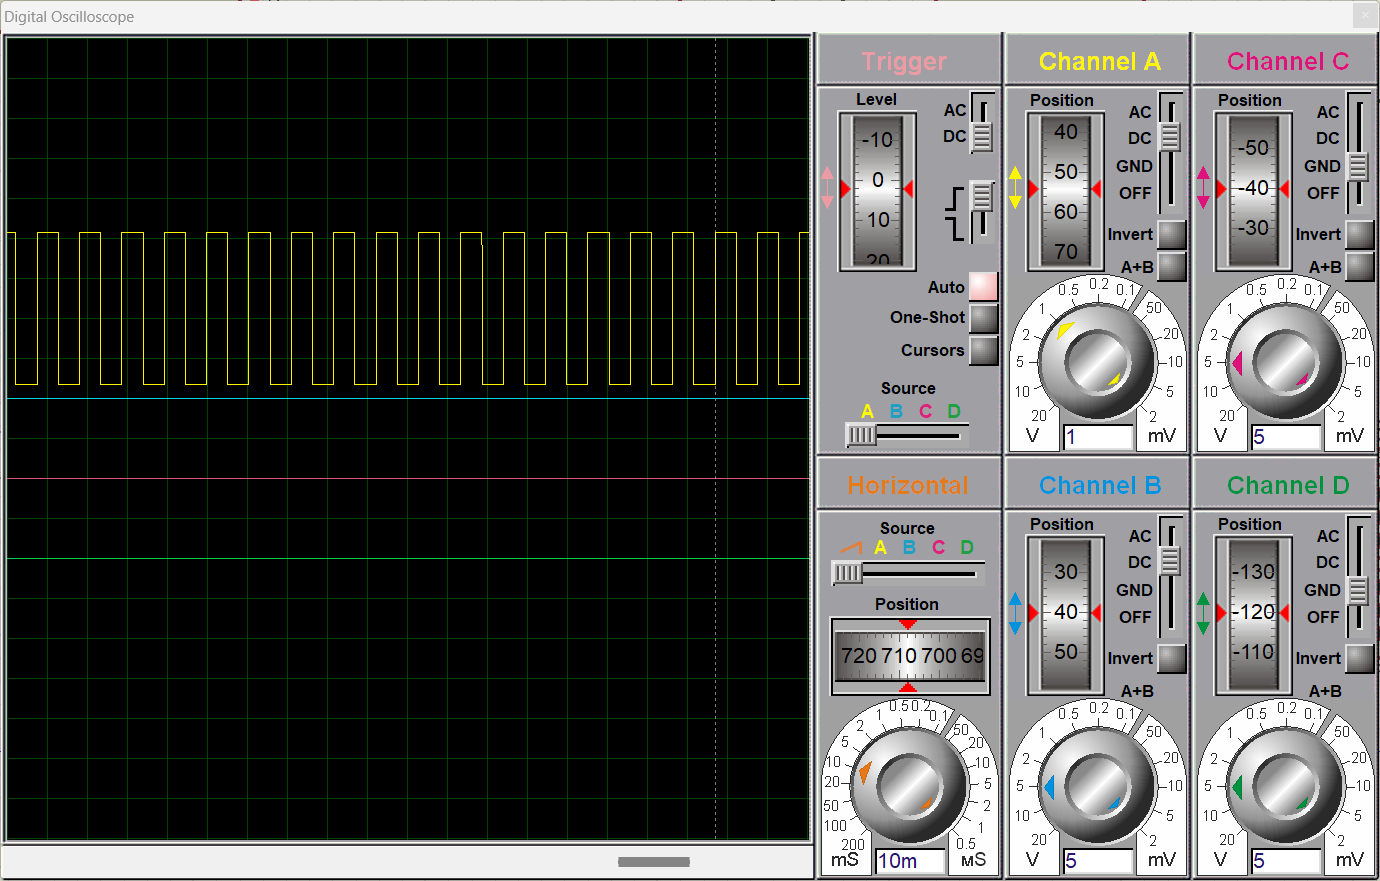
\includegraphics[width=\textwidth]{images/wave_square.png}
    \caption{方波输出}
  \end{subfigure}
  \hfill
  \begin{subfigure}{0.48\textwidth}
    \centering
    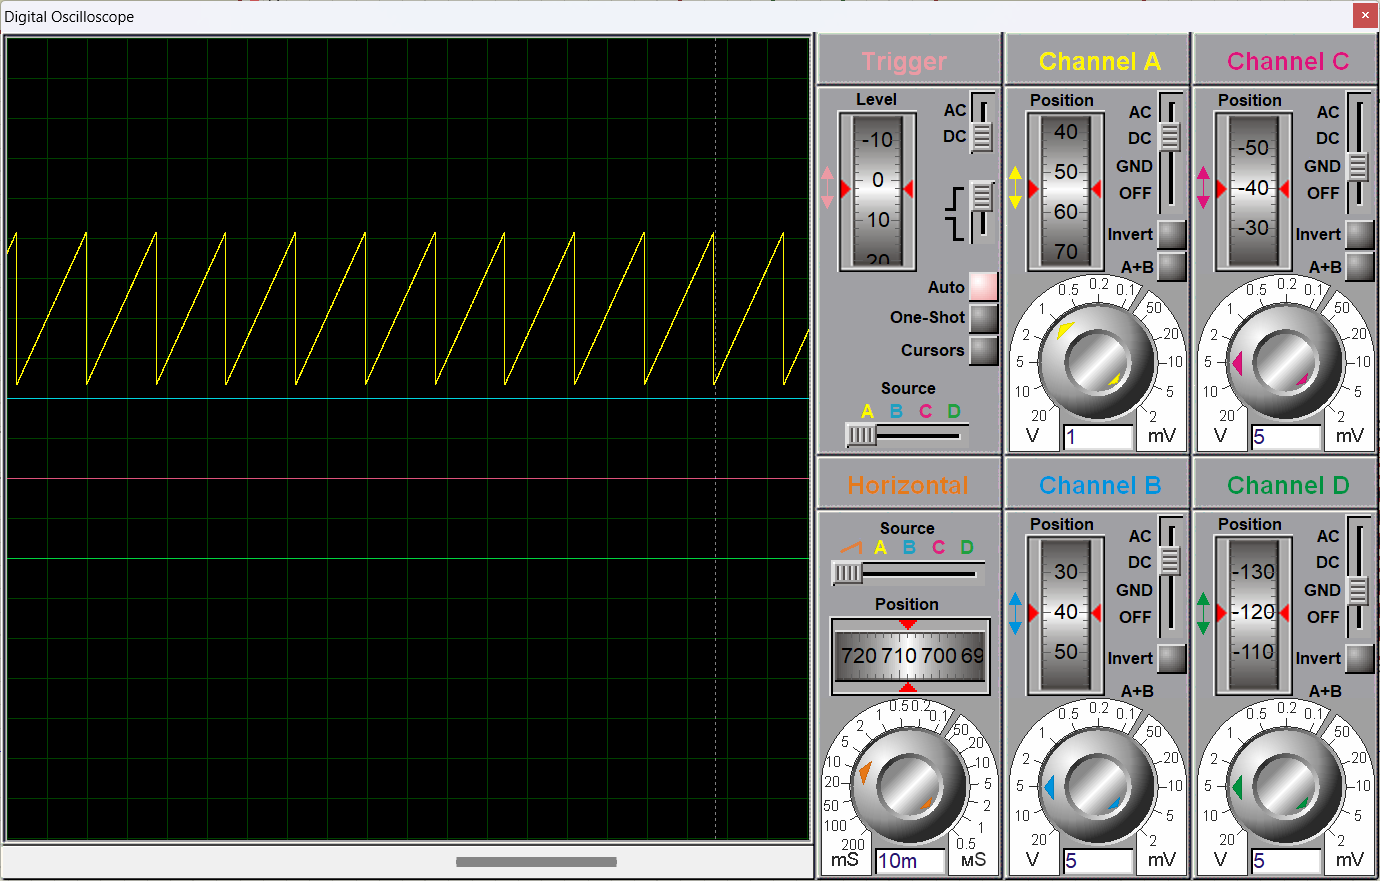
\includegraphics[width=\textwidth]{images/wave_sawtooth.png}
    \caption{锯齿波输出}
  \end{subfigure}

  \vspace{0.6em}
  \begin{subfigure}{0.48\textwidth}
    \centering
    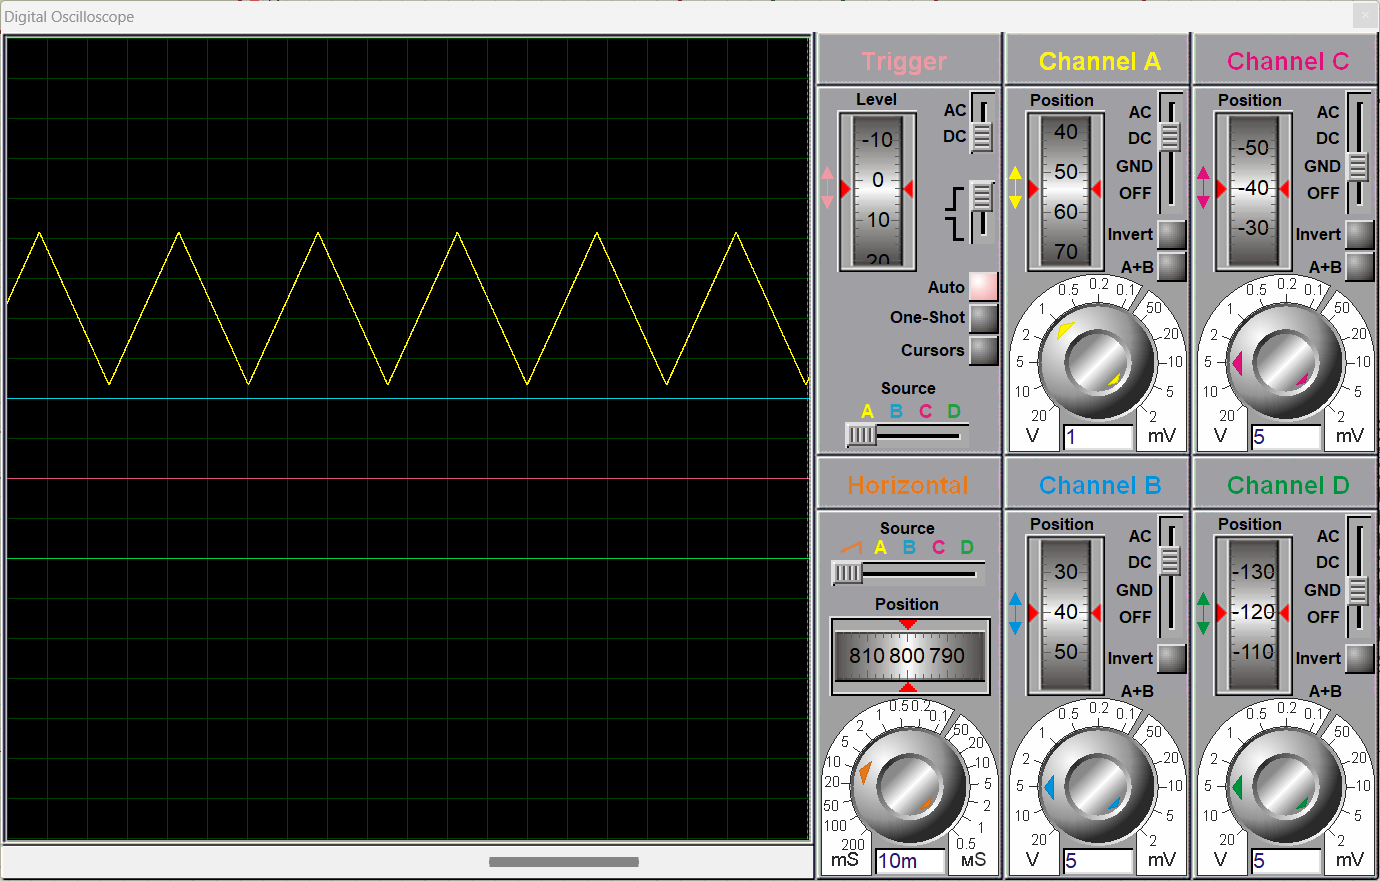
\includegraphics[width=\textwidth]{images/wave_triangle.png}
    \caption{三角波输出}
  \end{subfigure}
  \hfill
  \begin{subfigure}{0.48\textwidth}
    \centering
    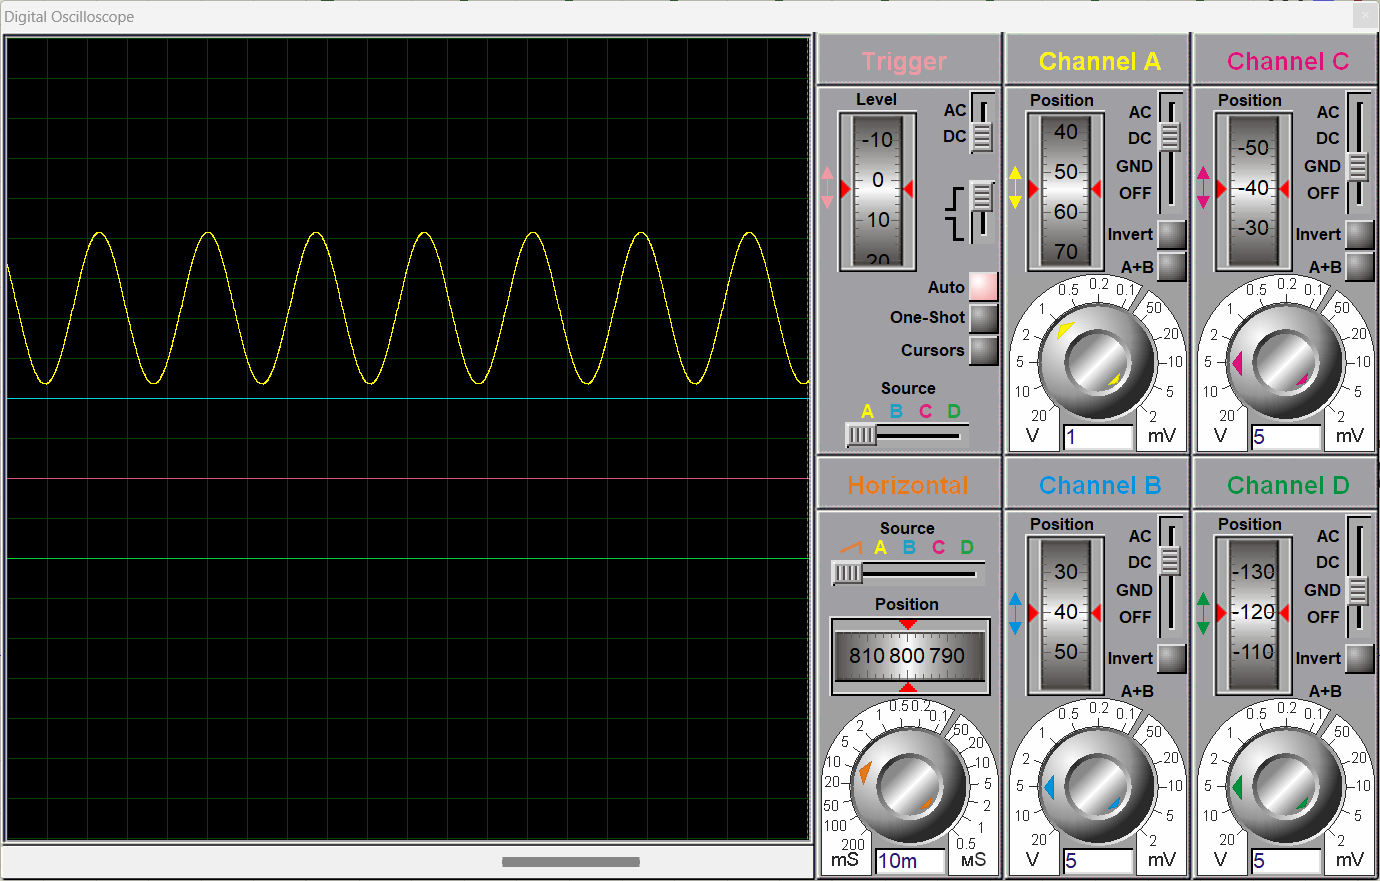
\includegraphics[width=\textwidth]{images/wave_sine.png}
    \caption{正弦波输出}
  \end{subfigure}
  \caption{四种波形的示波器仿真结果}
\end{figure}

从示波器截图可以看出，方波在高低电平之间快速切换，锯齿波呈现线性上升后跳变回零，三角波具有近似对称的上升和下降边沿，正弦波则表现为连续平滑的周期曲线。四种波形均与程序输出规律一致。

\subsection{频率调节对比}
\begin{figure}[H]
  \centering
  \begin{subfigure}{0.32\textwidth}
    \centering
    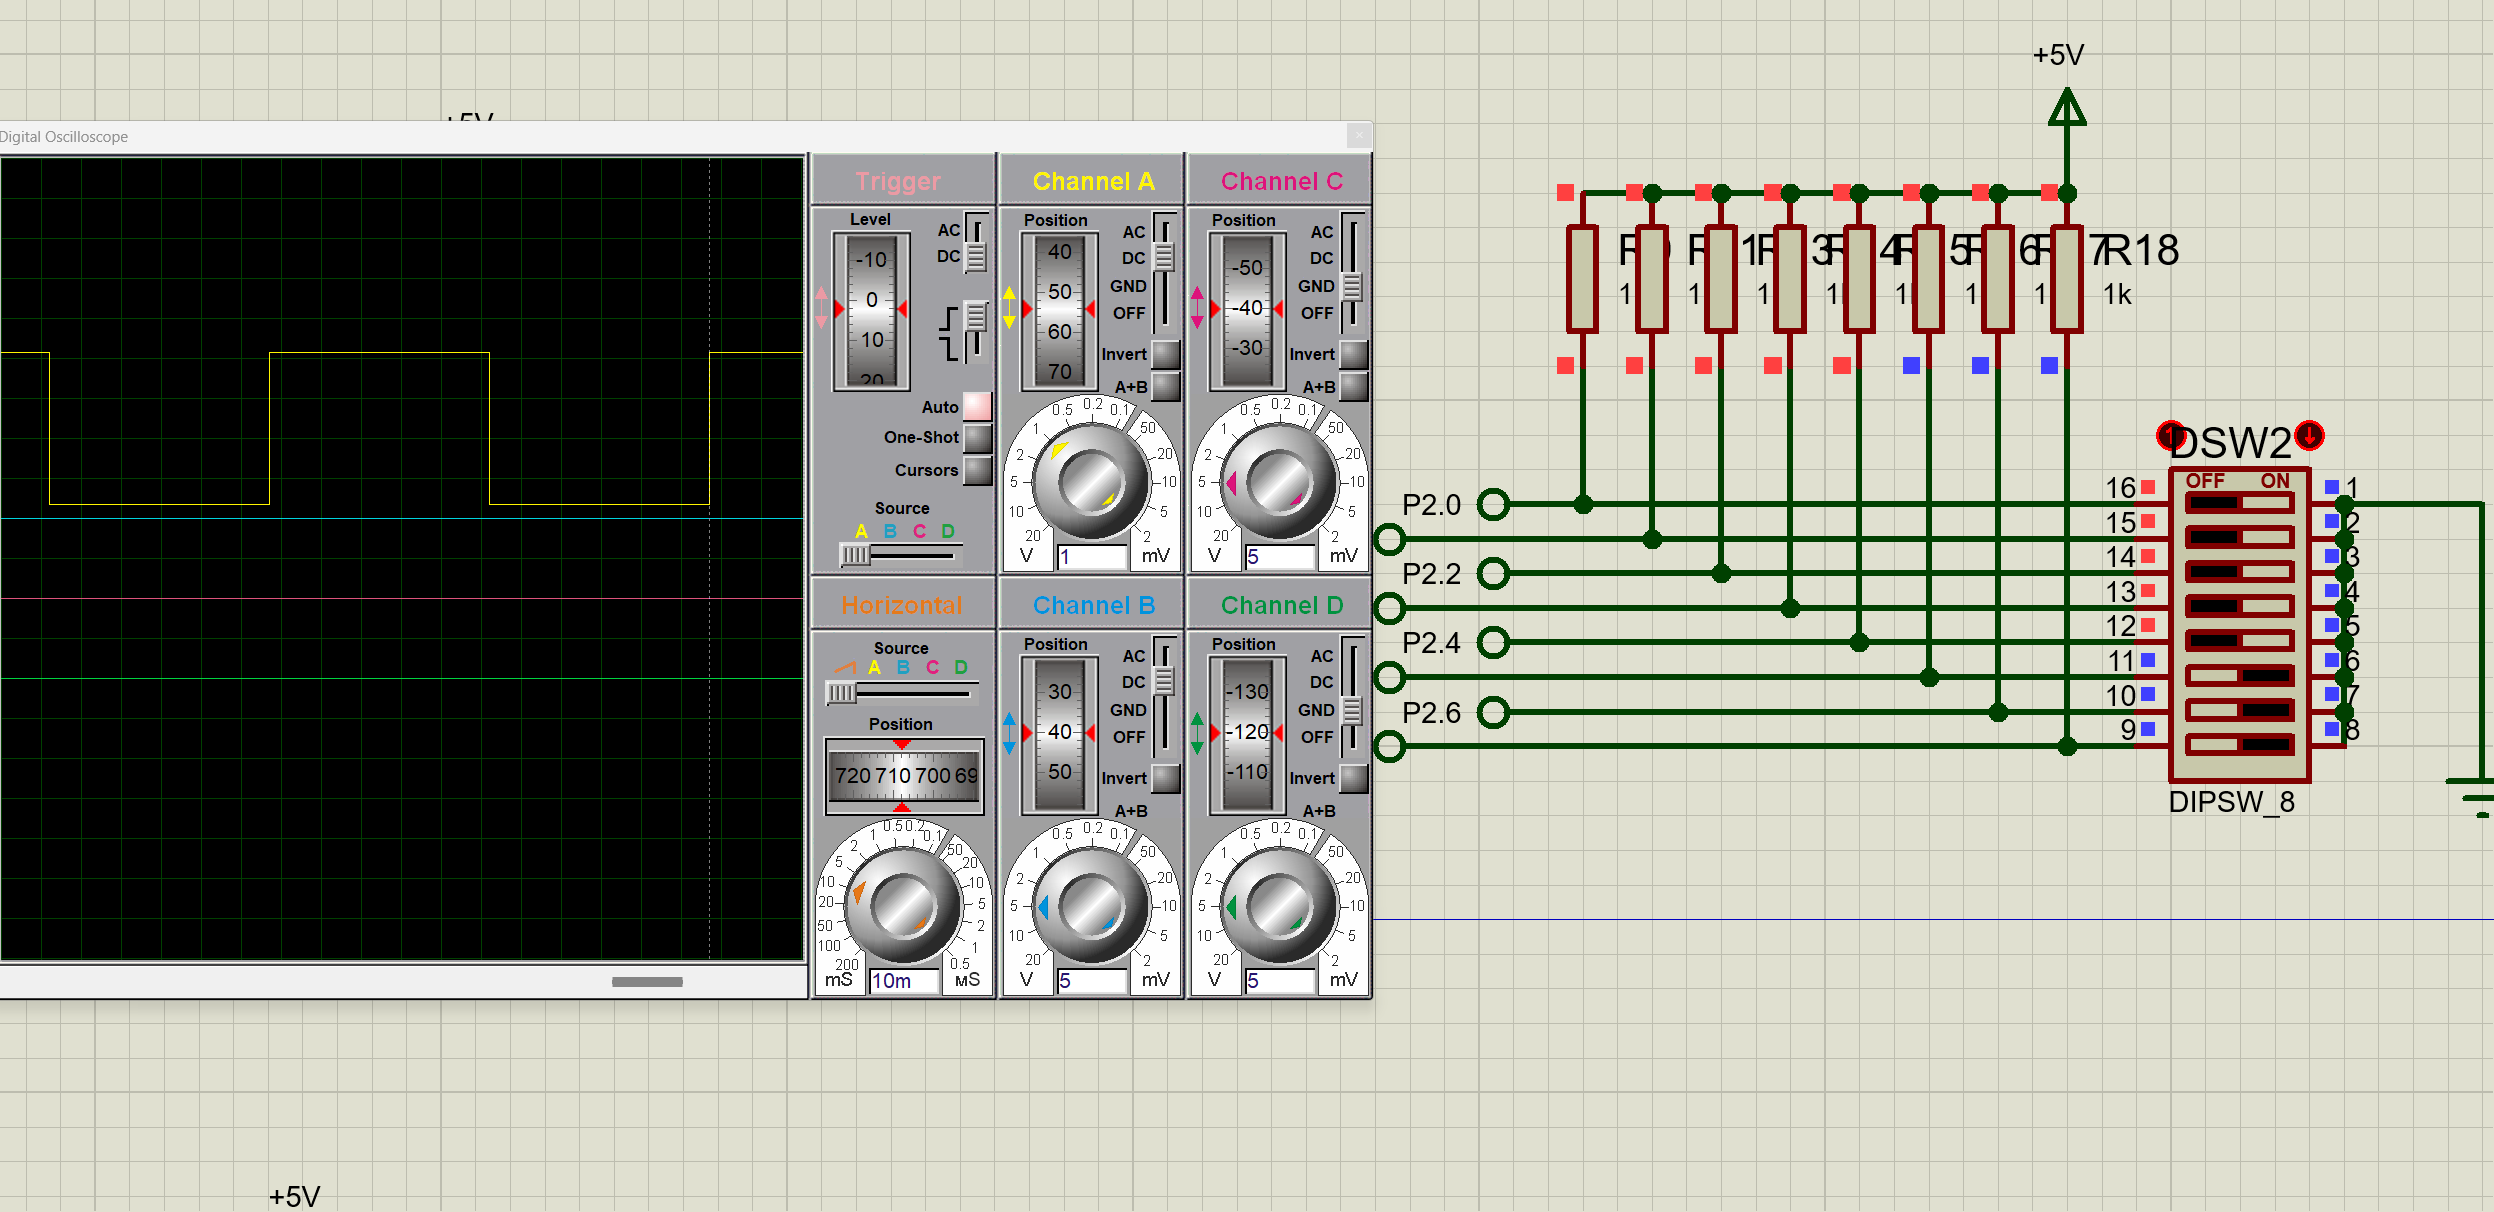
\includegraphics[width=\textwidth]{images/freq_low.png}
    \caption{低频输出}
  \end{subfigure}
  \hfill
  \begin{subfigure}{0.32\textwidth}
    \centering
    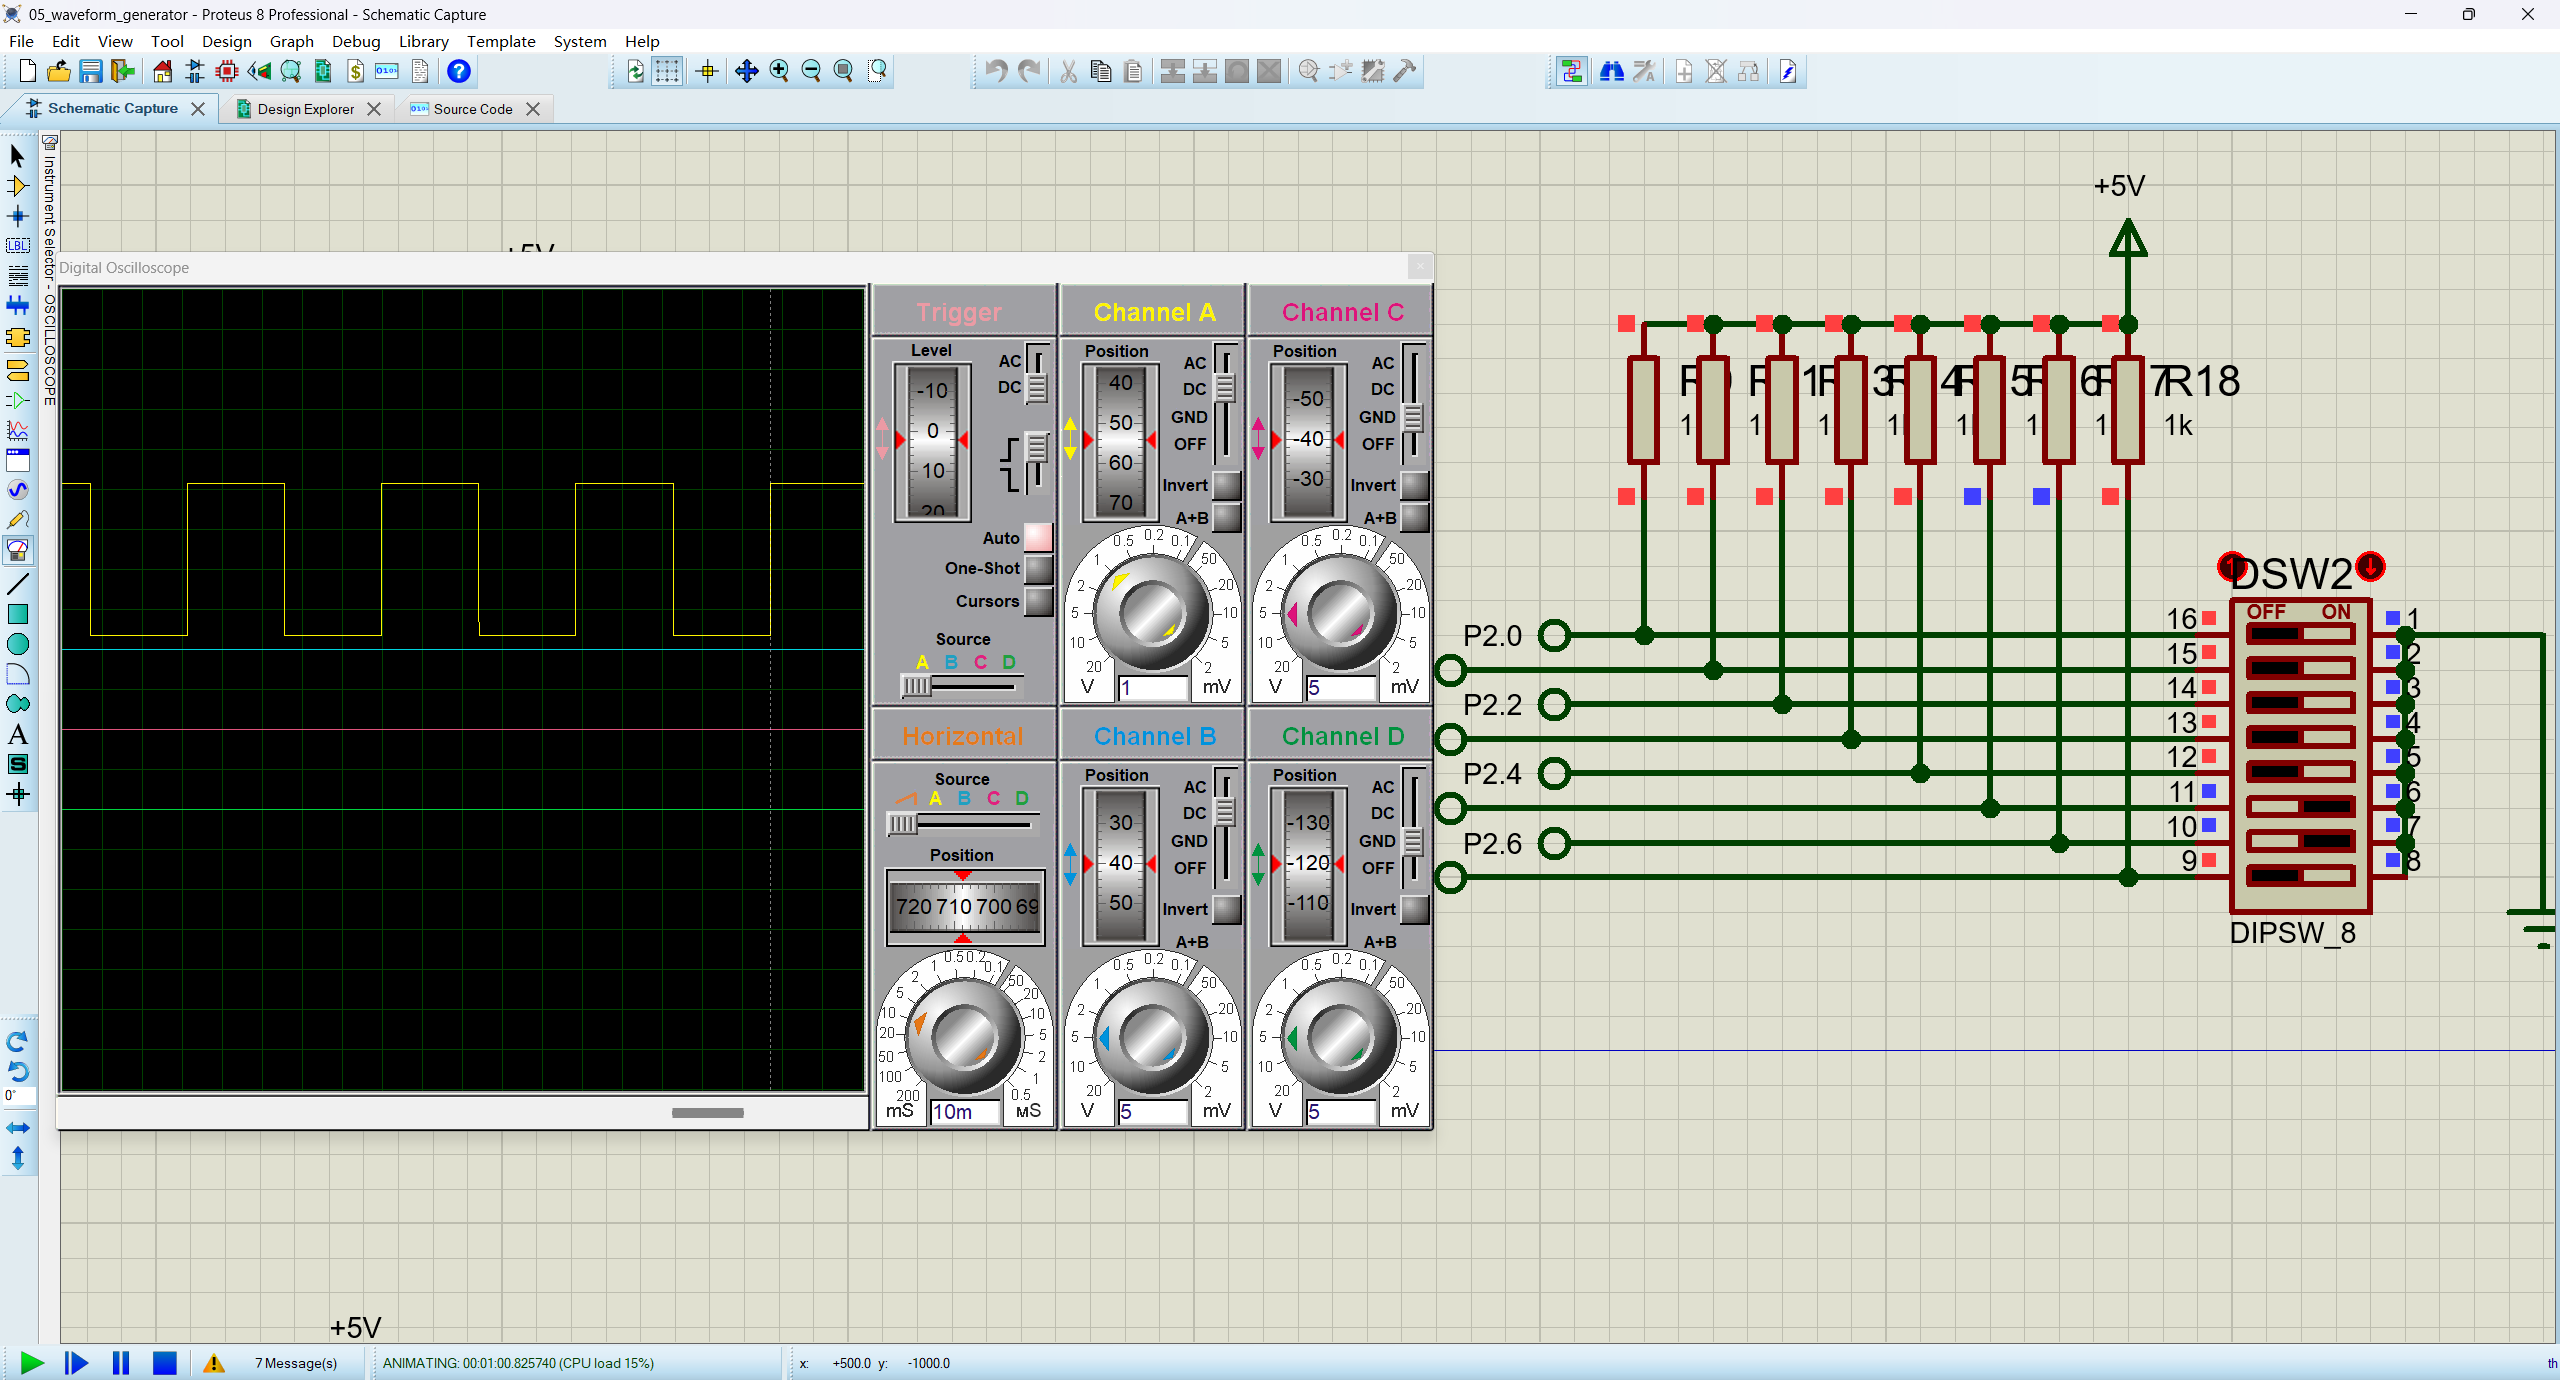
\includegraphics[width=\textwidth]{images/freq_mid.png}
    \caption{中频输出}
  \end{subfigure}
  \hfill
  \begin{subfigure}{0.32\textwidth}
    \centering
    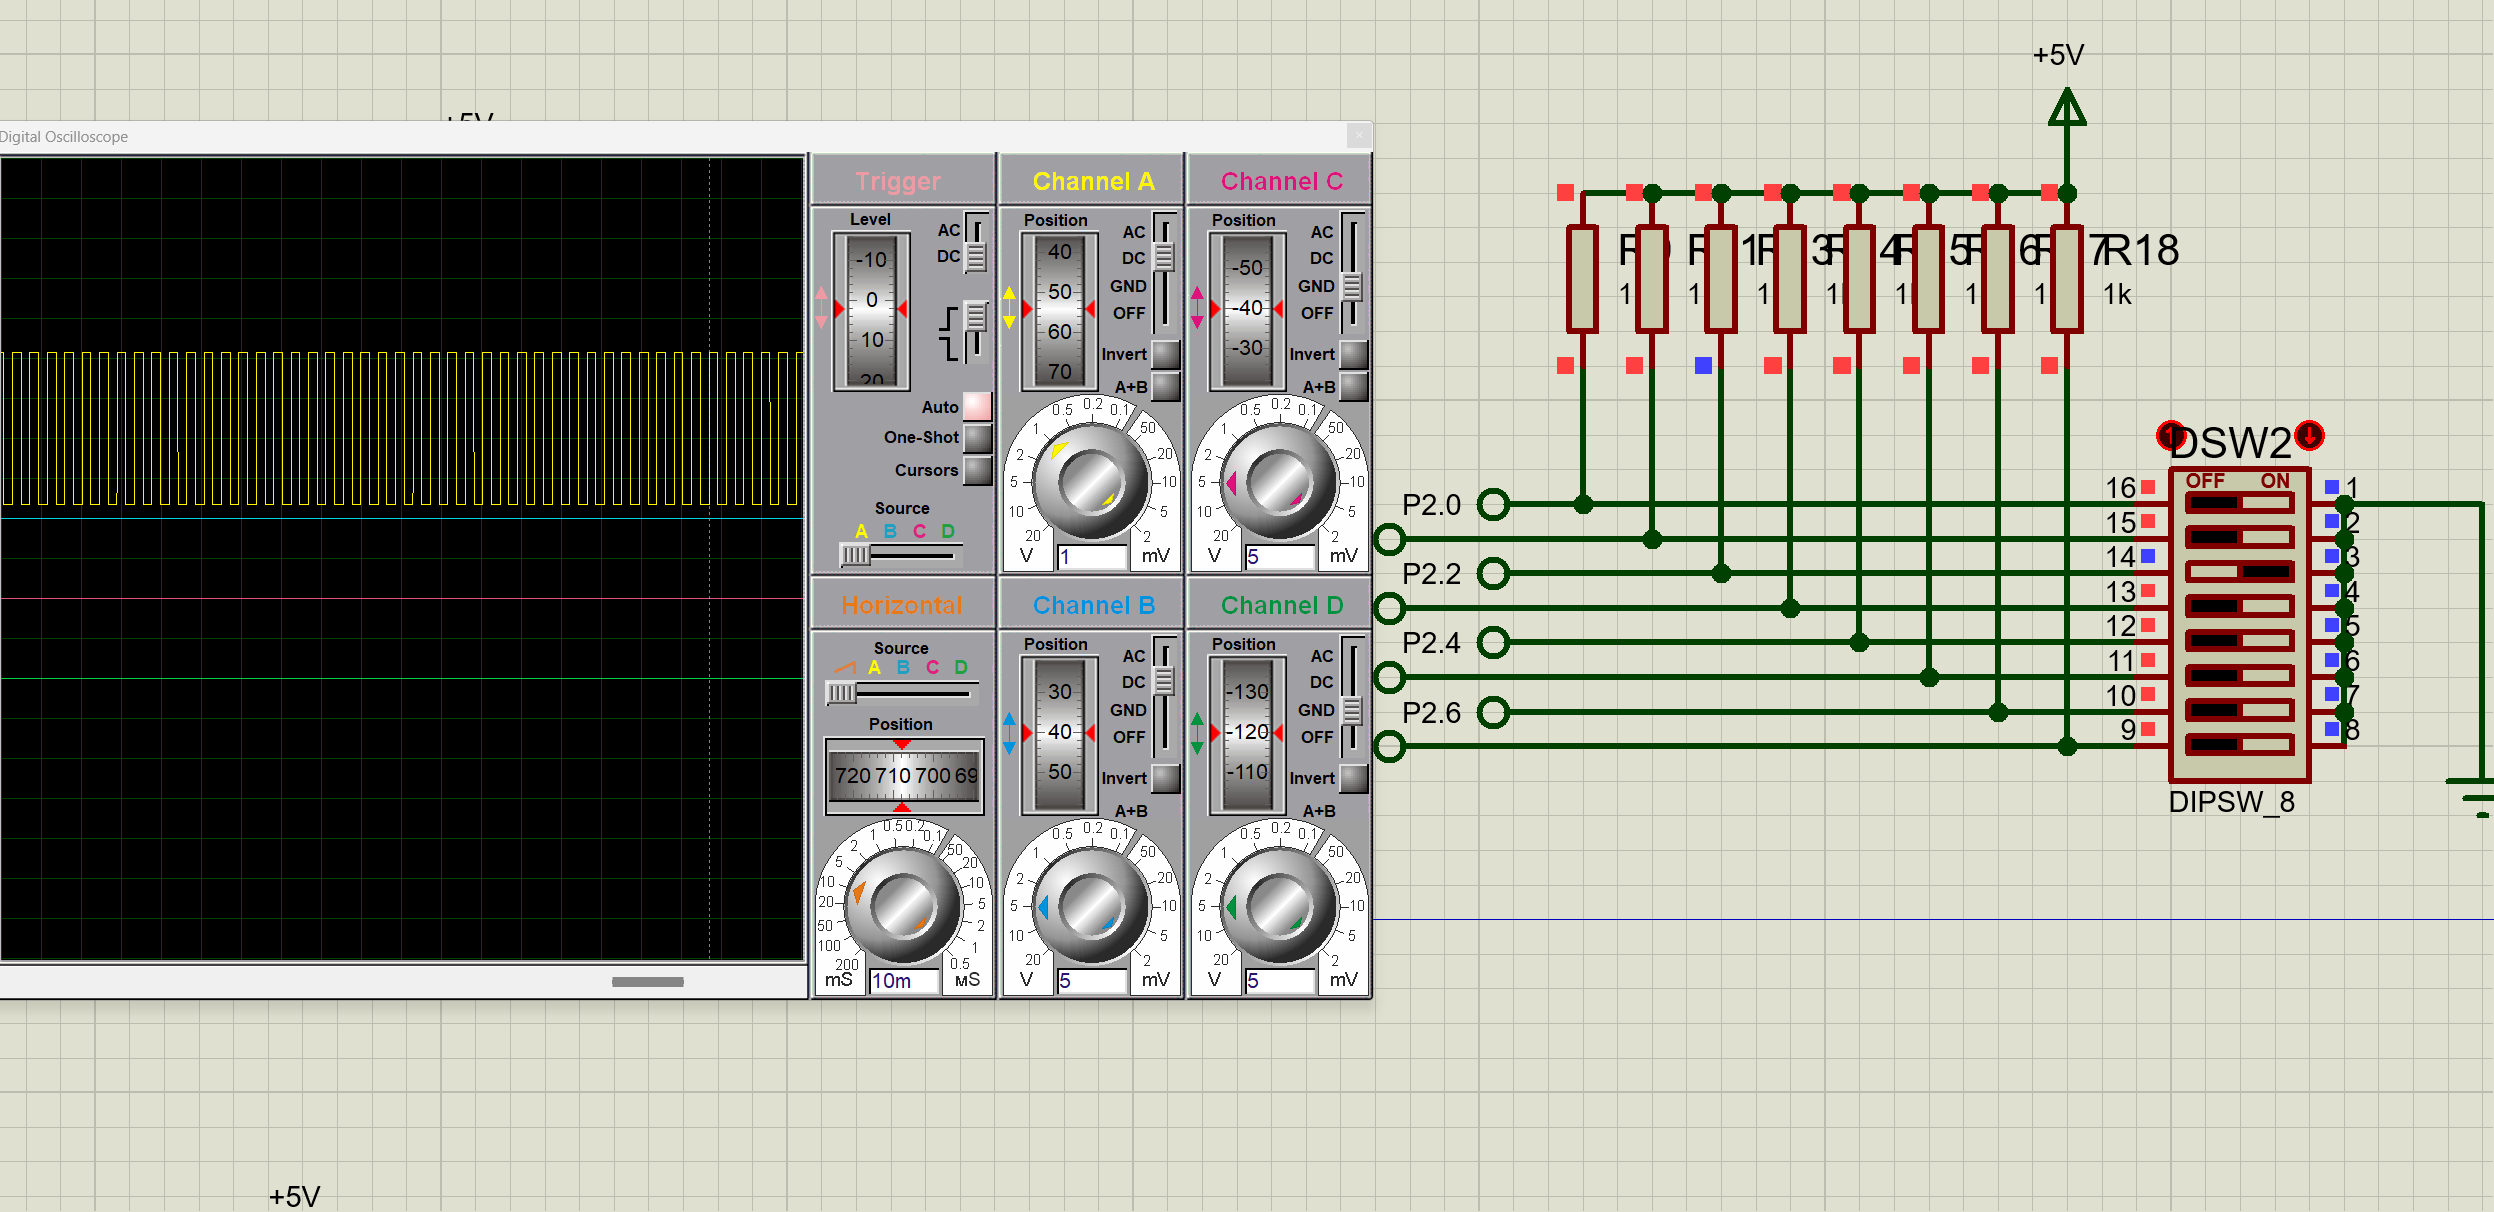
\includegraphics[width=\textwidth]{images/freq_high.png}
    \caption{高频输出}
  \end{subfigure}
  \caption{不同 P2 取值下的频率调节效果}
\end{figure}

频率对比结果表明，调节 P2 口拨码值后，同一屏幕时间范围内显示的周期数发生明显变化。低频时波形周期长、分布较稀疏；高频时周期变短、波形更密集，说明 P2 口频率控制逻辑有效。

\subsection{结果验证表}
\begin{table}[H]
  \centering
  \caption{波形发生器仿真结果记录}
  \renewcommand{\arraystretch}{1.35}
  \begin{tabular}{clcc}
    \toprule
    序号 & 测试内容 & 预期现象 & 结果 \\
    \midrule
    1 & 上电复位与默认状态 & 未按键时默认输出方波 & 符合 \\
    2 & 方波选择 & 输出高低电平交替的方波，P1.4 LED 点亮 & 符合 \\
    3 & 锯齿波选择 & 输出线性上升并回零的锯齿波，P1.5 LED 点亮 & 符合 \\
    4 & 三角波选择 & 输出线性上升再下降的三角波，P1.6 LED 点亮 & 符合 \\
    5 & 正弦波选择 & 输出平滑正弦曲线，P1.7 LED 点亮 & 符合 \\
    6 & P2 频率调节 & P2 值增大时输出频率升高 & 符合 \\
    \bottomrule
  \end{tabular}
\end{table}

\section{问题分析与改进建议}
\begin{enumerate}
  \item 当前频率调节依赖软件延时，延时期间 CPU 不能处理其他任务，且实际频率受指令执行时间影响。若需要更稳定的频率，可使用定时器中断产生固定采样节拍。
  \item DAC0832 采用直通方式，电路简单、便于实验观察，但如果后续需要与多路外设共享数据总线，可以改用锁存控制方式，提高总线时序的可控性。
  \item P1 口同时承担开关输入和 LED 输出，程序需要注意写端口时保持低四位为 1。若硬件资源允许，可以将输入和指示灯分配到不同端口，降低端口复用带来的软件约束。
  \item 正弦波由 92 点四分之一表生成，曲线已经较平滑。若追求更高精度，可增加表点数量；若追求更高频率，可减少表点或使用定时器配合查表输出。
  \item 机械拨码开关在实际硬件中可能存在抖动。本实验在 Proteus 中影响较小，若移植到实物系统，可增加简单消抖或在周期结束时多次确认输入状态。
\end{enumerate}

\section{实验结论}
本实验完成了基于 AT89C51、DAC0832 和 LM324 的波形发生器设计与仿真。系统通过 P0 口输出数字采样值，经 DAC0832 和运算放大器转换为模拟电压；通过 P1 口选择方波、锯齿波、三角波和正弦波，并用 LED 指示当前波形；通过 P2 口改变软件延时，实现输出频率调节。仿真结果显示，四种波形形状清晰，频率变化效果明显，硬件连接和软件控制逻辑均满足实验要求。
